\section{Webserver} \label{sec:Webserver}
Der Webserver bietet die Möglichkeit der Verwaltung des Spiels, der Abgabe von Flags sowie der Durchführung von Käufen im Flagshop und Challenges. Auch können Informationen zum Spiel, wie Einstellungen, Spielstand, Strafen und Teilnehmer abgerufen werden.

\subsection{Verwendung mehrerer Microservices}
Der Webserver kann nach dem Architekturmuster Microservices implementiert werden. Hierbei besteht die Anwendung aus mehreren unabhängig Komponenten, welche, sofern dies notwendig ist, untereinander kommunizieren. Die Komponenten sind so klein wie möglich und können jederzeit durch eine andere Implementierung ausgetauscht werden. \cite{wolffMicroservicesGrundlagenFlexibler2015} 

So wären die verschiedenen Komponenten des Webservers (Flagabgabe, Nutzerverwaltung, Spielsteuerung, etc.) unabhängig voneinander und können leichter weiterentwickelt oder ersetzt werden.

Die Verwendung dieses Architekturmusters wird bei der aktuellen Aufgabenstellung nicht angewendet, da durch die Entwicklung der vielen Einzelkomponenten ein zu hoher Aufwand für zu geringen Nutzen entstehen würde.

\subsection{Fat Webserver}
Der Webserver beinhaltet sowohl die Logik als auch die Darstellung. Bei einer Anfrage an den Webserver wird eine Antwort bestimmt und diese dann in eine Vorlage beziehungsweise ein HTML Dokument eingebettet. Danach wird die Antwort zurück an den Anfragenden gesendet.

Während der Implementierung des Prototyps und des weiteren Entwurfs hat sich ein Problem mit dem Flagshop Login herausgestellt.

Für die Nutzung des Flagshops ist ein Multi-Login notwendig, da nur am Webserver eingeloggte Nutzende sich mit einem extra angelegten Account am Flagshop anmelden und diesen verwenden dürfen. Dieser Multi-Login ließ sich mit dem im Prototypen implementierten Session basierten Login nicht einfach umsetzen. 

So ist für diesen Anwendungsfall ein Stateless Login besser geeignet, da hier die benötigten Informationen vom Client, je nach Anliegen, gesendet werden können. 

Die Nutzung des Stateless Logins bietet die Perspektive der Verwendung eines Stateless \linebreak Webservers sowie eines Thin Webservers. Bei einem Thin Webserver werden nur Daten und keine Repräsentation an dem Client zurückgesendet. So wird die Aufgabe der Darstellung der Daten an den Client übertragen.

Durch die Nutzung eines Thin Servers werden zwei Dinge ermöglicht. 

Zum Ersten ist es möglich, den Client und Server unabhängig voneinander zu entwickeln, zu verändern und zu verbessern. Damit kann in Zukunft eine Iteration der Software einfacher geschehen. Zweitens können die Studierenden eigene Clients programmieren, um mit der Anwendung zu interagieren.

\subsection{Thin Webserver}
\begin{center}
	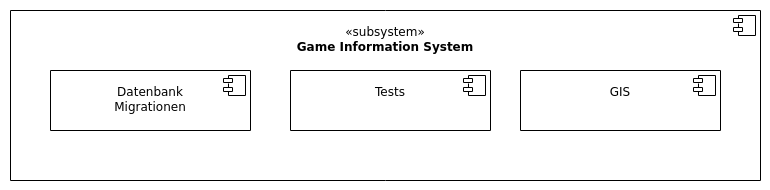
\includegraphics[width=\linewidth]{entwurf/gis/comp-gis}
	\captionof{figure}{REST Interface im Überblick (Komponentendiagramm)}
\end{center}

Der Server besteht aus der Komponente \textit{Game Information System}, welche wiederum aus drei weiteren Komponenten besteht. 

Die Komponente \textit{GIS} implementiert die gesamte Server Logik. In diesem Modul wird der eigentliche Thin Server, über den die teilnehmenden und betreuenden Personen mit der Anwendung interagieren können, implementiert.

In der Komponente Datenbank Migrationen sind Migrationsskripts hinterlegt, die die Datenbank Iterationen festhalten. Diese Skripts sollen genutzt werden, um die verwendete Datenbanken einfach mit dem benötigten Schema zu initialisieren. 

Die letzte Komponente beinhaltet Unit-Tests. Mithilfe der implementierten Unit-Tests kann die Funktionalität der Anwendung bei späteren Änderungen überprüft werden.

Da der Thin Server nur eine Brücke zwischen Nutzenden und Scanner oder Datenbank darstellt, kann von einer API (Application Programming Interface) gesprochen werden. Mithilfe dieser API können beispielsweise der aktuelle Spielstand aus der Datenbank ausgelesen und Strafen eingetragen werden.

\subsubsection{API}
Um bei der Implementierung der API einem Standard zu folgen, wird der de facto Standard für HTTP-APIs Representational State Transfer (REST) verwendet.

Ein RESTful Interface ermöglicht, dass Ressourcen auf dem Webserver eindeutig identifizierbar sind, damit diese als Ziel von Operationen ausgewählt werden können. Des Weiteren werden einheitliche Schnittstellen genutzt. Dazu müssen Standardmethoden und -repräsentationen verwendet werden. \cite{beimsWebApplikationenREST2014}

Durch diese Anforderungen bietet das REST Interface die Möglichkeiten, alle zur Verfügung stehenden Ressourcen auf die gleiche Art und Weise zu verwalten. Außerdem wird mit dieser Herangehensweise die HTTP-Methode GET nicht länger zur Veränderung oder Erschaffung von Ressourcen verwendet, sondern die dafür ausgelegten HTTP-Methoden. Die für die Verwendung benötigten Daten werden auch nicht länger als Parameter der Anfrage beigefügt, sondern im Body der Anfrage übertragen. \cite{beimsWebApplikationenREST2014}

Alle Routen werden mit dem Versionspräfix \textit{/v1} versehen. Diese Versionierung soll bei späteren Iterationen der API Kollisionen verhindern und die Nutzung der alten Versionen weiterhin ermöglichen. 

Bei der Implementierung sollen die zur Verfügung stehenden HTTP Methoden benutzt werden. Das REST-Interface soll auch mit entsprechenden HTTP Codes antworten, um die Antwort und den Erfolg einer Anfrage auch ohne Antworttext interpretieren zu können. Bei der Datenübertragung zwischen Client und Server soll das JavaScript Object Notation (JSON) Format für die Formatierung der gesendeten Daten verwendet werden.

\begin{table}
	\centering
	\begin{tabular}{c c}
		GET & Auf Ressourcen zugreifen \\ 
		POST & Neue Ressourcen erzeugen \\  
		PUT & Bestehende Ressourcen verändern \\
		DELETE & Vorhandene Ressourcen löschen \\
	\end{tabular}
	\caption{Übersicht über die verwendeten HTTP Methoden}
	\label{table:http-methods}
\end{table}

Neben den in \autoref{table:http-methods} aufgezeigten Methoden gibt es noch weitere HTTP Methoden, welche keine Anwendung in dem zu implementierenden REST-Interface erhalten.

\subsection{Funktionale Eigenschaften}
\subsubsection{Login}\label{subsub:login}
\begin{center}
	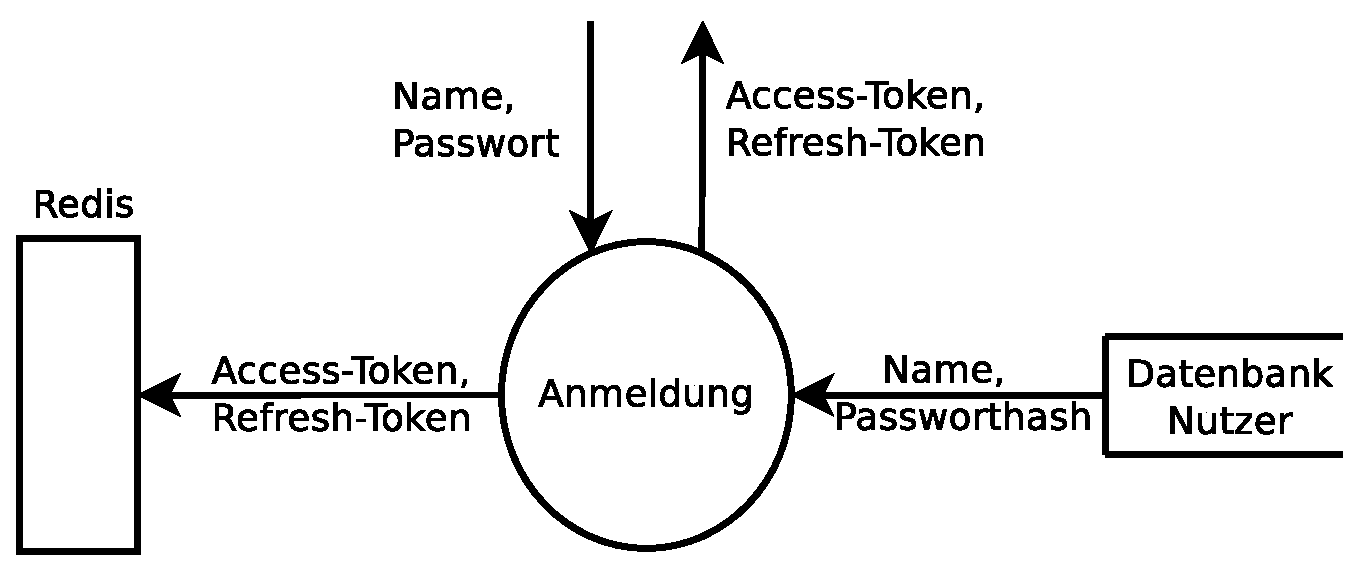
\includegraphics[width=100mm]{entwurf/gis/dfd-gis-login}
	\captionof{figure}{Datenfluss während eines Logins (Datenflussdiagramm)}
\end{center}

Bei einem Login sendet der Nutzende die Kombination aus Nutzernamen und Passwort in seiner Anfrage an den Webserver. Sollte der Nutzername und das Passwort mit den in der Datenbank gespeicherten Informationen übereinstimmen, wird ein Access- und ein Refresh-Token ausgestellt. Wichtig hierbei ist, dass das Passwort in der Datenbank \textbf{nur} im gehashten Format vorliegt.

Sollte kein Hackitzugang benötigt werden, muss für die Ausstellung der Tokens kein Nutzername und Passwort angegeben werden.

\begin{center}
	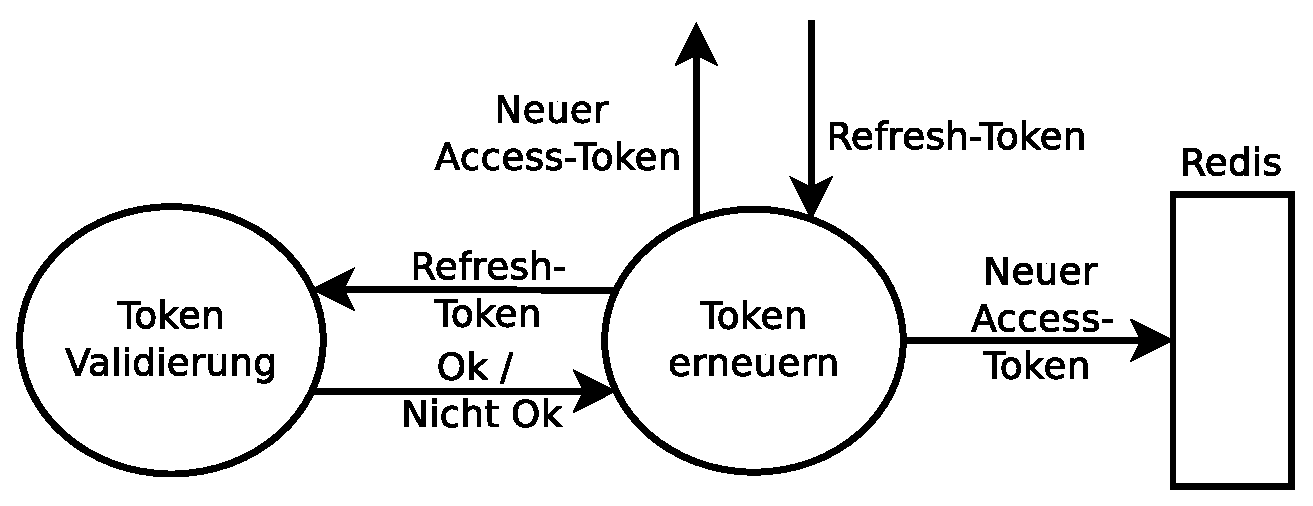
\includegraphics[width=100mm]{entwurf/gis/dfd-gis-token-refresh}
	\captionof{figure}{Datenfluss während eines Logins mit Refresh Token (Datenflussdiagramm)}
\end{center}

Ein Refresh-Token wird ausgestellt, da beide Token eine begrenzte Lebenszeit haben. Der Refresh-Token hat eine längere Lebenszeit und ermöglicht die erneute Ausstellung eines \linebreak Access-Tokens ohne Angabe eines Nutzernamens und Passwortes.

Des Weiteren werden alle ausgestellten Token für die Dauer der Gültigkeit in der Redis-Datenbank gespeichert, um diese bei späteren Anfragen zu validieren. 

\subsubsection{Authentifizierung}
\begin{center}
	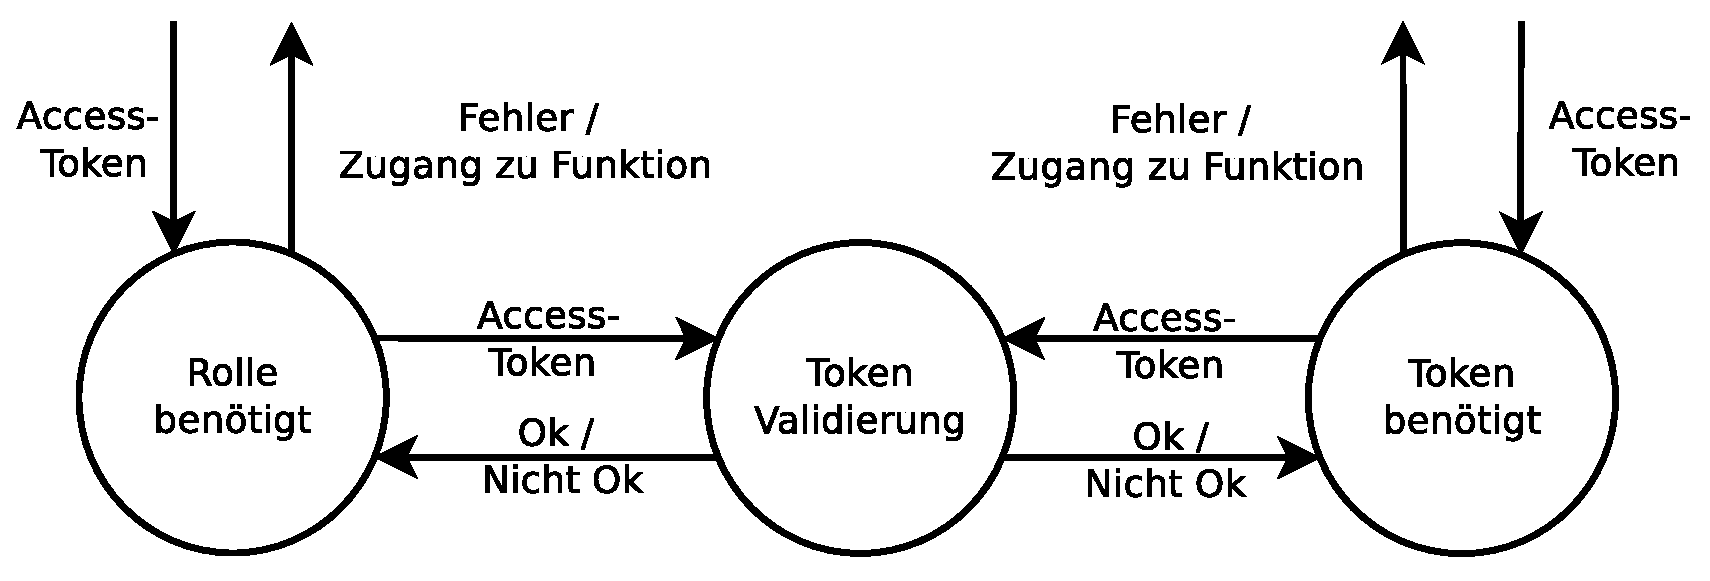
\includegraphics[width=100mm]{entwurf/gis/dfd-gis-role-token}
	\captionof{figure}{Datenfluss der Authentifizierung und Autorisierung (Datenflussdiagramm)}
\end{center}

Die Authentifizierung des Benutzers wird über die in \autoref{subsub:login} erwähnten Tokens realisiert. Die Tokens müssen vom Client bei jeder Anfrage mitgesendet werden und enthalten neben der Nutzerkennung weitere Informationen zu Berechtigungen. 

Dies reduziert die Anfragen an die Datenbank. Nachteil hierbei sind langsame Änderungen der Berechtigungen, da die neuen Berechtigungen erst mit dem Erstellen eines neuen Tokens übernommen werden. Da Änderungen an der Berechtigung selten vorkommen, kann dieser Nachteil relativiert werden.

Mit den im Token codierten Berechtigungen kann der Server die Autorisierung der vom Nutzenden angefragten Aktion durchführen.

\paragraph{Tokenvalidierung}
\begin{center}
	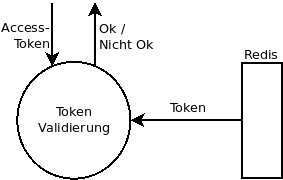
\includegraphics[width=55mm]{entwurf/gis/dfd-gis-token-validation}
	\captionof{figure}{Datenfluss während der Tokenvalidierung (Datenflussdiagramm)}
\end{center}

Für die Authentifizierung und Autorisierung müssen die mitgesendeten Token validiert werden.
Dazu erhalten diese einen Zeitstempel der Ausstellung und des Ablaufs und eine Signatur, die eine Manipulation verhindern soll. Führt der Nutzende einen Logout durch, wird der Token in der Datenbank als widerrufen markiert. 

\subsubsection{Registierung von GameClients}
\begin{center}
	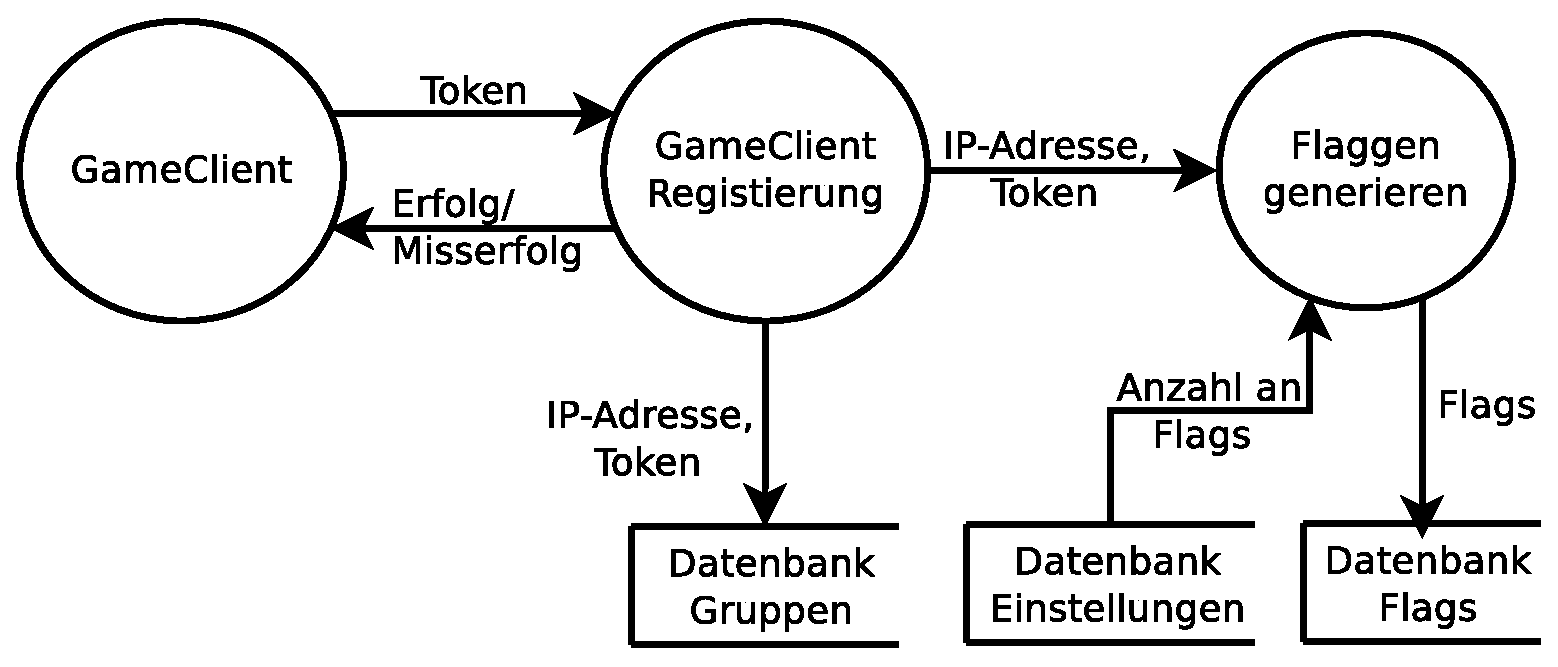
\includegraphics[width=100mm]{entwurf/gis/dfd-gis-registierung}
	\captionof{figure}{Datenfluss der Registrierung (Datenflussdiagramm)}
\end{center}

Die teilnehmenden GameClients sollen aufgrund der Anforderung nicht länger fest in der Anwendung vorliegen, sondern dynamisch hinterlegt werden. Deshalb müssen die GameClients sich vor Spielstart registrieren.

\paragraph{Flaggenerierung}
Durch die benötigte Registrierung ist es möglich, dass der Algorithmus zur Flaggenerierung verändert wird. Dies soll geschehen, damit die Flags nicht länger pro Semester, sondern im besten Fall für immer, einzigartig sind.

Damit die Flags einzigartig sind, überträgt der GameClient einen Token bei der Registrierung. Dieser wird sowohl vom GameClient als auch vom Server genutzt, um die benötigten Flags zu generieren.

Die Idee, dass die Flaggenerierung nur auf dem Server stattfindet, wurde verworfen, da die nutzende Person auf dem Client die Möglichkeit hat die Flags bei der Übertragung abzufangen und abzugeben. Eine Verschlüsselung oder andere Verfahren würden keinen Mehrwert in puncto Sicherheit liefern, da die nutzende Person Root-Rechte auf ihrem System hat. Eine Verschlüsselung der Flags mit dem PGP-Verfahren bringt keinen wirklichen Mehrwert, daauf den vorhandene PGP-Key zugreifen werden kann. 

\subsubsection{Flagabgabe}

Da die Flag Abgabe einen Hauptteil des Versuchs darstellt, müssen authentifizierte Spielende die auf dem eigenen oder gegnerischen System gefundene Flags abgeben können.

Das GIS muss die abgegebene Flag auf Gültigkeit prüfen und entweder Offensiv- und \linebreak
Defensiv- oder Discoverpunkte verrechnen. Auch muss sichergestellt werden, dass eine Gruppe eine Flag nur einmal abgeben kann.

Gruppen können alle eigenen Flags sowie gegnerische Flags, welche auf den GameClients verteilt sind, abgeben. Gegnerische Flagshop Flags können nicht abgegeben werden, da diese als nicht schützenswert betrachtet werden.

Ob die Abgabe im Angriffszeitraum geschieht muss geprüft werden. Andernfalls soll die Abgabe nicht weiter verarbeitet werden und bei einer Abgabe während der Discoverzeit soll eine Strafe ausgesprochen werden.


\subsubsection{Spielsteuerung}

Die Betreuenden sollen über das GIS das Spiel steuern können. Dabei müssen sie in der Lage sein, ein Spiel zu starten, zu pausieren und zu beenden. Die Steuerung des Scanners soll an das Spiel gekoppelt werden, aber auch eigenständig funktionieren.

Des Weiteren sollen die betreuenden Personen die Möglichkeit besitzen, Strafen an Gruppen, welche die Regeln gebrochen haben, verteilen zu können. Hier muss die Gruppe, der Grund der Bestrafung sowie die Anzahl der Strafpunkte übermittelt werden.

\subsubsection{Accountverwaltung}

Administrierende und Betreuungspersonal sollen die Möglichkeit erhalten, neue Accounts anzulegen, zu bearbeiten und zu löschen. Wichtig hierbei ist, dass das Betreuungspersonal nur Accounts der Rolle Player verwalten kann.

Außerdem ist ein Import der Studierendenzugänge zu realisieren, damit die generierten Zugänge einfach übernommen werden können.

\subsubsection{Spielstände}

Die abgespeicherten Spielstände sollen über das GIS abrufbar sein. Hierzu soll zuerst eine Liste der verfügbaren Spielstände inklusive des Datums der Speicherung an den Anfragenden übermittelt werden. Mit dieser Liste kann der benötigte Spielstand ermittelt und im nächsten Schritt angefragt werden. 

Dieser detaillierte Spielstand beinhaltet die Punkte aller teilnehmenden Gruppen, die überwachten Schwachstellen und Dienste sowie den Spielstatus.

\subsubsection{Steuerung der Services}

Die betreuenden Personen des Versuchs, sollen die Möglichkeit erhalten einzelne \linebreak
Scan-Operationen zu (de-)aktivieren ohne, dass eine Änderung an der Software vorgenommen werden muss. Die Gewichtung der einzelnen Services soll jederzeit änderbar sein.

\subsubsection{Einstellungen}

Die betreuenden Personen sollen die Einstellungen des Spiels verändern können. Die Spieleinstellungen sollen als Key-Value-Paar vorliegen. Zu den Einstellungen zählen beispielsweise die Anzahl der generierten Flags pro Gruppe, aber auch, ob ein anonymer Login für die Rolle \textit{Player} vorgesehen ist.

\subsubsection{Notizen}

Den betreuenden Personen soll es möglich gemacht werden permanente Hinweise zu geben. Des Weiteren sollen sie in der Lage sein, bestehende Hinweise zu bearbeiten oder zu löschen.

Studierende können die verfassten Notizen einsehen, um Hinweise oder Anweisungen zum Versuch zu erhalten.

\subsubsection{Flagshop}
\begin{center}
	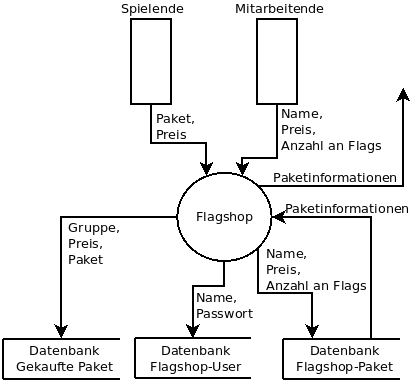
\includegraphics[width=120mm]{entwurf/gis/dfd-gis-flagshop}
	\captionof{figure}{Datenfluss im Flagshop (Datenflussdiagramm)}
\end{center}

Der Flagshop muss die Verwaltung von Flagshop-Usern und Flagshop-Paketen sowie einen Kauf der Flagshop-Pakete ermöglichen.

Flagshop-User können durch die teilnehmenden Teams erstellt werden. Für die Erstellung werden Flags an die Gruppe verteilt. Betreuende Personen können ebenfalls für Gruppen Flagshop-User erstellen. Des Weiteren ist es ihnen möglich, bestehende Flagshop-User zu ändern und zu löschen.

Außerdem müssen Flagshop-Pakete durch die Betreuenden verwaltet werden. Die Erstellung von Flagshop-Paketen soll nur vor einem Spielstart möglich sein, damit die richtige Anzahl an Flags bei der Registrierung eines GameClients erzeugt werden kann. Die Flagshop-Pakete sollen neben den Kosten und dem Namen auch die Anzahl der erwerbbaren Flags enthalten.

Studierende können Flagshop-Pakete erwerben. Die Besonderheit hierbei soll sein, dass diese den Kaufpreis mitsenden und so die Flagshop-Pakete für einen anderen Preis als angegeben erwerben können.

\subsubsection{Challenges}
\begin{center}
	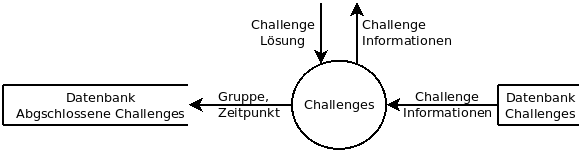
\includegraphics[width=110mm]{entwurf/gis/dfd-gis-challenge}
	\captionof{figure}{Datenfluss der Challenges (Datenflussdiagramm)}
\end{center}

Die Studierenden müssen Informationen zu Challenges sowie deren Ablageort abrufen können. Des Weiteren sollen sie in der Lage sein die Challenges abzuschließen. Hierfür teilen die Challenges am Ende ein Passwort mit, welches ebenfalls in der Datenbank vorhanden ist. Die Studierenden können dieses Passwort dann als Beweis der Lösung der Challenge an das GIS übermitteln.

Die Challenges werden von einem Webserver zur Verfügung gestellt werden. Sie werden nicht über das GIS verteilt, da dies als API nur Daten und keine Ressourcen an den Client übermittelt.

\subsection{Reverse Proxy}
Für das Betreiben wird auf den bereits im EZS Labor verwendeten Apache HTTP-Server zurückgegriffen. Durch die Entscheidung bleibt dieser als einziger Einstiegspunkt für Anfragen zuständig. So kann die Protokollierung der Anfragen sowie die Verschlüsselung der Verbindung an die Webserver Software abgegeben werden.

Der Reverse Proxy muss bei der Weiterleitung der Anfrage an das GIS sicherstellen, dass die eigentliche IP-Adresse der Anfrage dem GIS zugänglich ist. Dies wird benötigt, um die zugehörige Gruppe, bei der Registrierung und dem Login zu bestimmen. Die originale IP-Adresse der Anfrage soll in einen HTTP Header gespeichert werden.

In einen HTTP Header können Server und Client zusätzliche Informationen zur Anfrage oder Antwort beifügen. \cite{mdncontributorsHTTPHeaders2020}

Um einen Spoofing-Angriff zu erschweren und das Vertrauen in den Header mit der IP-Adresse zu erhöhen, soll ein weiterer Header mit einem Geheimnis gesetzt werden. Anhand dieses Geheimnisses kann das GIS entscheiden, ob die Anfrage über einen vertrauenswürdigen Proxy weitergeleitet oder ob ein Spoofing-Angriff durchgeführt worden ist. Die Erweiterung wird benötigt, da die Anwendung auch ohne einen Reverse Proxy betrieben werden kann. In diesem Anwendungsfall kann die angreifende Person sich als Proxy für eine andere Gruppe ausgeben.

Bei einem Spoofing-Angriff versendet die angreifende Person Anfragen für andere IP-Adressen und erhält die Antwort. So könnte diese im Namen anderer agieren und den Angegriffenen beispielsweise Minuspunkte verschaffen.